\documentclass[12pt,a4paper]{article}
\usepackage[utf8]{inputenc}
\usepackage[english]{babel}
\usepackage{amsmath}
\usepackage{amsfonts}
\usepackage{amssymb}
\usepackage{graphicx}
\usepackage{listings}
\lstset{language=ml}
\lstset{commentstyle=\textit}
\lstset{mathescape=true}
\lstset{backgroundcolor=,rulecolor=}
\lstset{frame=single}
\lstset{breaklines=true}
\lstset{basicstyle=\footnotesize\ttfamily}
\DeclareMathOperator{\tick}{tick}
\DeclareMathOperator{\step}{step}
\DeclareMathOperator{\wait}{wait}
\DeclareMathOperator{\yield}{yield}
\DeclareMathOperator{\id}{id}
\DeclareMathOperator{\owner}{owner}
\DeclareMathOperator{\local}{local}
\DeclareMathOperator{\remote}{remote}
\DeclareMathOperator{\localconnect}{localconnect}
\DeclareMathOperator{\remoteconnect}{remoteconnect}
\DeclareMathOperator{\letlet}{let}
\DeclareMathOperator{\letin}{in}
\DeclareMathOperator{\send}{send}
\DeclareMathOperator{\receive}{receive}
\DeclareMathOperator{\sendRel}{send\_reliable}
\DeclareMathOperator{\receiveMany}{receive\_many}


\begin{document}
\title{Communicating parallel games}
\author{M. Abbadi \and A. Cortesi \and F. Di Giacomo \and A. Plaat \and P. Spronck \and D. Dini \and G. Costantini \and G. Maggiore}
\maketitle

\section{Introduction}
\label{sec:introduction}
The number of programming languages available on the market has dramatically increased during the last years. The tiobe index \cite{tiobe2018}, a ranking of programming languages based on their popularity, lists 50 programming languages for 2018. This number is only a small glimpse of the real amount, since it does not take into account several languages dedicated to specific applications. This growth has brought a further need for new compilers that are able to translate programs written in those languages into executable code. The goal of this work is to investigate how the development speed of a compiler can be boosted by employing meta-compilers, programs that generalize the task performed by a normal compiler. In particular the goal of this research is creating a meta-compiler that significantly reduces the amount of code needed to define a language and its compilation steps, while maintaining acceptable performance.

This chapter introduces the issue of expressing the solution of problems in terms of algorithms in Section \ref{sec:ch1_algorithms}. Then we proceed by defining how the semi-formal definition of an algorithm must be translated into code executable by a processor (Section \ref{sec:ch1_programming_languages}). In this section we discuss the advantages and disadvantages of using different kinds of programming languages with respect to their affinity with the specific hardware architecture and the scope of the domain they target. In Section \ref{sec:ch1_compilers} we explain the reason behind compilers and we explain why building a compiler is a time-consuming task. In Section \ref{sec:ch1_metacompilers} we introduce the idea of meta-compilers as a further step into generalizing the task of compilers. In this section we also explain the requirements, benefits, and the relevance as a scientific topic. Finally in Section \ref{sec:ch1_problem_statement} we formulate the problem statement and the research questions that this work will answer.

\section{Algorithms and problems}
\label{sec:ch1_algorithms}
Since the ancient age, there has always been the need of describing the sequence of activities needed to perform a specific task \cite{barbin2012history}, to which we refer with the name of \textit{Algorithm}. The allegedly most ancient known example of this dates back to the Ancient Greek, when Hero invented an algorithm to perform the factorization and the approximation of the square root, discovered also by other civilizations \cite{ bailey2012ancient, smith1923history} . Regardless of the specific details of each algorithm, one needs to use some kind of language  to define the sequence of steps to perform. In the past people used natural language to describe such steps but, with the advent of the computer era, the choice of the language has been strictly connected with the possibility of its implementation. Natural languages are not suitable for the implementation, as they are known to be verbose and ambiguous \cite{church1982coping, resnik1999semantic}. For this reason, several kind of formal solutions have been employed, which are described below.

\subsubsection*{Flow charts}
A flow chart is a diagram where the steps of an algorithm are defined by using boxes of different kinds, connected by arrows to define their ordering in the sequence. The boxes are rectangular-shaped if they define an \textit{activity} (or processing step), while they are diamond-shaped if they define a \textit{decision}. A rectangle with rounded corners denotes the initial step. An example of a flow chart describing how to sum the numbers in a sequence is described in Figure \ref{fig:ch1_flow_chart}.

\begin{figure}
	\centering
	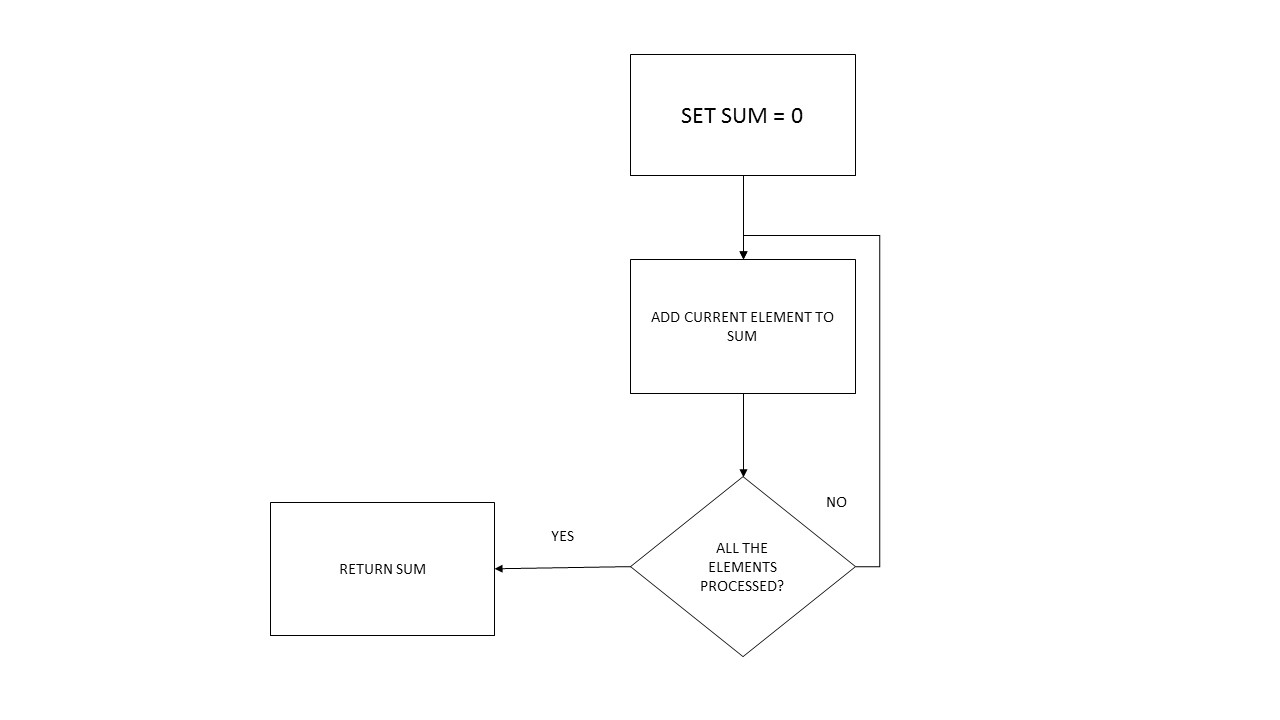
\includegraphics[width = \textwidth]{Figures/flow_chart}
	\caption{Flow chart for the sum of a sequence of numbers}
	\label{fig:ch1_flow_chart}
\end{figure}

\subsubsection*{Pseudocode}
Pseudocode is a semi-formal language that might contain also statements expressed in natural language and omits system specific code like opening file writers, printing messages on the standard output, or even some data structure declaration and initialization. It is intended mainly for human reading rather than machine reading. The pseudocode to sum a sequence of numbers is shown in Algorithm \ref{alg:ch1_pseudocode}.

\begin{algorithm}
	\caption{Pseudocode to perform the sum of a sequence of integer numbers}
	\label{alg:ch1_pseudocode}
	\begin{algorithmic}
		\Function{SumIntegers}{$l \text{ list of integers}$}
			\State $sum \gets 0$
			\ForAll {$x \text{ in } l$}
				\State $sum \gets sum + x$
			\EndFor
			\State \Return $sum$
		\EndFunction
	\end{algorithmic}
\end{algorithm}

\subsubsection*{Advantages and disadvantages}
Using flow charts or pseudo-code has the advantage of being able to define an algorithm in a way which is very close to the abstractions employed when using natural language: a flow chart combines both the use of natural language and a visual interface to describe an algorithm, pseudo-code allows to employ several abstractions and even define some steps in terms of natural language. The drawback of these two formal representations is that, when it comes to the implementation, the definition of the algorithm must be translated by hand into code that the hardware is able to execute. This could be done by implementing the algorithm in a low-level or high-level programming language. This process affects at different levels how the logic of the algorithm is presented, as explained further.

\section{Programming languages}
\label{sec:ch1_programming_languages}
A programming language is a formal language that is used to define instructions that a machine, usually a computer, must perform in order to produce a result through computation \cite{mordechai1996, narasimhan1967programming, oxford2008}. There is a wide taxonomy used to classify programming languages depending on their use \cite{kelleher2005lowering, myers1986visual, myers1990taxonomies}, but all can be grouped according to two main characteristics: the level of abstraction, or how close to the specific targeted hardware they are, and the domain, which defines the range of applicability of a programming language. In the following sections we give an exhaustive explanation of the aforementioned characteristics.

\subsection{Low-level programming languages}
\label{subsec:ch1_ll_languages}
A low-level programming language is a programming language that provides little to no abstraction from the hardware architecture of a processor. This means that it is strongly connected with the instruction set of the targeted machine, the set of instructions a processor is able to execute. These languages are divided into two sub-categories: \textit{first-generation} and \textit{second-generation} languages:

\subsubsection*{First-generation languages}
\textit{Machine code} falls into the category of first-generation languages. In this category we find all those languages that do not require code transformations to be executed by the processor. These languages were used mainly during the dawn of computer age and are rarely employed by programmers nowadays. Machine code is made of stream of binary data, that represents the instruction codes and their arguments \cite{guide2011intel, seal2001arm}. Usually this stream of data is treated by programmers in hexadecimal format, which is then remapped into binary code. The programs written in machine code were once loaded into the processor through a front panel, a controller that allowed the display and alteration of the registers and memory (see Figure \ref{fig:ch1_front_panel}). An example of machine code for a program that computes the sum of a sequence of integer numbers can be seen in Listing \ref{lst:ch1_machine_code}.

\begin{figure}
	\centering
	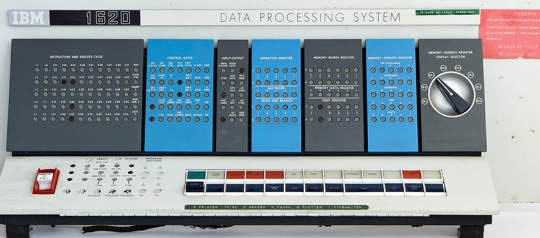
\includegraphics[width = \textwidth]{Figures/ch1_front_panel}
	\caption{Front panel of IBM 1620}
	\label{fig:ch1_front_panel}
\end{figure}

\begin{minipage}{\linewidth}
\begin{lstlisting}[numbers = left, caption = Machine code to compute the sum of a sequence of numbers, label = lst:ch1_machine_code]
 00075	c7 45 b8 00 00
 00 00
 0007c	eb 09	
 0007e	8b 45 b8
 00081	83 c0 01
 00084	89 45 b8
 00087	83 7d b8 0a
 0008b	7d 0f
 0008d	8b 45 b8
 00090	8b 4d c4
 00093	03 4c 85 d0
 00097	89 4d c4
 0009a	eb e2
\end{lstlisting}
\end{minipage}

\subsubsection*{Second-generation languages}
The languages in this category provides an abstraction layer over the machine code by expressing processor instructions with mnemonic names both for the instruction code and the arguments. For example, the arithmetic sum instruction \texttt{add} is the mnemonic name for the instruction code \texttt{0x00} in \texttt{x86} processors. Among these languages we find \textit{Assembly}, that is mapped with an \textit{Assembler} to machine code. The Assembler can load directly the code or link different \textit{object files} to generate a single executable by using a \textit{linker}. An example of assembly \texttt{x86} code corresponding to the machine code in Listing \ref{lst:ch1_machine_code} can be found in Listing \ref{lst:ch1_assembly_code}. You can see that the code in the machine code \texttt{00081	83 c0 01} at line 5 has been replaced by its mnemonic representation in Assembly as \texttt{add	eax, 1}.

\begin{minipage}{\linewidth}
\begin{lstlisting}[numbers = left, caption = Assembly x86 code to compute the sum of a sequence of numbers, label = lst:ch1_assembly_code]
mov	DWORD PTR _i$1[ebp], 0
jmp	SHORT $LN4@main
$LN2@main:
mov	eax, DWORD PTR _i$1[ebp]
add	eax, 1
mov	DWORD PTR _i$1[ebp], eax
$LN4@main:
cmp	DWORD PTR _i$1[ebp], 10			; 0000000aH
jge	SHORT $LN3@main
mov	eax, DWORD PTR _i$1[ebp]
mov	ecx, DWORD PTR _sum$[ebp]
add	ecx, DWORD PTR _numbers$[ebp+eax*4]
mov	DWORD PTR _sum$[ebp], ecx
jmp	SHORT $LN2@main
\end{lstlisting}
\end{minipage}

\subsubsection*{Advantages and disadvantages}
Writing a program in low-level programming languages might produce programs that are generally more efficient than their high-level counterparts, as ad-hoc optimizations are possible. However, the high-performance comes at great costs: (\textit{i}) the programmer must be an expert of the underlying architecture and of the specific instruction set of the processor, (\textit{ii}) the program loses portability because the low-level code is tightly bound to the specific hardware architecture it targets, (\textit{iii}) the logic and readability of the program is hidden among the details of the instruction set itself, and (\textit{iv}) developing a program in assembly requires a considerable effort in terms of time and debugging \cite{frampton2009demystifying}: assembly lacks any abstraction from the concrete hardware architecture, such as a type system, that partially ensures the correctness of the program or high-level constructs that allow to manipulate the execution of the program.

\subsection{High-level programming languages}
\label{subsec:ch1_hl_languages}
A high-level programming language is a programming language that offers a high level of abstraction from the specific hardware architecture of the machine. Unlike machine code (and in some way also assembly), high-level languages are not directly executable by the processor and they require some kind of translation process into machine code. The level of abstraction offered by the language defines how high level the language is. Several categories of high-level programming language exist, but the main one are described below.

\subsubsection*{Imperative programming languages}
\textit{Imperative programming languages} model the computation as a sequence of statements that alter the state of the program (usually the memory state). A program in such languages consists then of a sequence of \textit{commands}. Notable examples are FORTRAN, C, and PASCAL. An example of the program used in Listing \ref{lst:ch1_machine_code} and \ref{lst:ch1_assembly_code} written in C can be seen in Listing \ref{lst:ch1_c_code}. Line 5 to 9 corresponds to the Assembly code in Listing \ref{lst:ch1_assembly_code}.

\begin{lstlisting}[numbers = left, caption = C code to compute the sum of a sequence of numbers, label = lst:ch1_c_code]
int main()
{
  int numbers[10] = { 1, 6, 8, -2, 4, 3, 0, 1, 10, -5 };
  int sum = 0;
  for (int i = 0; i < 10; i++)
  {
    sum += numbers[i];
  }
  printf("%d\n", sum);
}
\end{lstlisting}

\subsection*{Declarative programming languages}
\textit{Declarative programming languages} are antithetical to those based on imperative programming, as they model computation as an evaluation of expressions and not as a sequence of commands to execute. Declarative programming languages are called as such when they are side-effects free or referentially transparent. The definition of referential transparency varies \cite{quine2013word}, but it is usually explained with the substitution principle, which states that a language is referentially transparent if any expression can be replaced by its value without altering the behaviour of the program \cite{mitchell2003concepts}. For instance, the following sentences in natural language are both true

\begin{lstlisting}
Cicero = Tullius

''Cicero`` contains six letters
\end{lstlisting} 

\noindent
but they are not referentially transparent, since replacing the last name with the middle name falsifies the second sentence.

A similar situation in programming languages is met when considering variable assignments: the statement

\begin{lstlisting}
x = x + 5
\end{lstlisting}

\noindent
is not referentially transparent. Let us assume this statement appears twice in a program and that at the beginning x = 0. Clearly the expression \texttt{x + 5} results in the value 5 the first time, but the second time the same statement is executed the expression has value 10. Thus replacing all the occurrences of \texttt{x + 5} with 5 is wrong, which is why imperative languages are not referentially transparent. A more rigorous definition of referential transparency can be found in \cite{sondergaard1990referential}.

Declarative programming languages are often compared to imperative programming languages by stating that declarative programming defines \textit{what} to compute and not \textit{how} to compute it. This family of languages include \textit{functional programming}, \textit{logic programming}, and \textit{database query languages}. Notable examples are F\#, Haskell, Prolog, SQL, and Linq (which is a query language embedded in C\#). Listing \ref{lst:ch1_fsharp_code_rec} shows the code to perform the sum of a sequence of integer numbers in F\# with a recursive function. Higher-order functions, such as \texttt{fold}, allow even to capture the same recursive pattern into a single function as shown in Listing \ref{lst:ch1_fsharp_code_fold}. Both implementations are referentially transparent.

\begin{lstlisting}[caption = Recursive F\# code to compute the sum of a sequence of numbers, label = lst:ch1_fsharp_code_rec]
let rec sumList l =
  match l with
  | [] -> 0
  | x :: xs -> x + (sumList xs)
\end{lstlisting}

\begin{lstlisting}[caption = F\# code to compute the sum of a sequence of numbers using higher-order functions, label = lst:ch1_fsharp_code_fold]
let sumList l = l |> List.fold (+) 0
\end{lstlisting}

\subsection{General-purpose vs Domain-specific languages}
\label{sec:ch1_dsl}
\textit{General-purpose languages} are defined as languages that can be used across different application domains and lack abstractions that specifically target elements of a single domain. Example of these are languages such as C, C++, C\#, and Java. Although several applications are still being developed by using general-purpose programming languages, in several contexts it is more convenient to rely on \textit{domain-specific languages}, because they offer abstractions relative to the problem domain that are unavailable in general-purpose languages \cite{van2000domain, voelter2013dsl}. Notable examples of the use of domain-specific languages are listed below.

\subsubsection*{Graphics programming}
Rendering a scene in a 3D space is often performed by relying on dedicated hardware. Modern graphics processors rely on shaders to create various effects that are rendered in the 3D scene. Shaders are written in domain-specific languages, such as GLSL or HLSL \cite{glhl2014, hlsl2018, hlslref2018}, that offer abstractions to compute operations at GPU level that are often used in computer graphics, such as vertices and pixel transformations, matrix multiplications, and interpolation of textures. Listing \ref{lst:ch1_hlsl_code} shows the code to implement light reflections in HLSL. At line 4 you can, for example, see the use of matrix multiplication provided as a language abstraction in HLSL.

\begin{lstlisting}[numbers = left, caption = HLSL code to compute the light reflection, label = lst:ch1_hlsl_code]
VertexShaderOutput VertexShaderSpecularFunction(VertexShaderInput input, float3 Normal : NORMAL)
{
  VertexShaderOutput output;
  float4 worldPosition = mul(input.Position, World);
  float4 viewPosition = mul(worldPosition, View);
  output.Position = mul(viewPosition, Projection);
  float3 normal = normalize(mul(Normal, World));
  output.Normal = normal;
  output.View = normalize(float4(EyePosition,1.0f) - worldPosition);
  return output;
}
\end{lstlisting}

\subsubsection*{Game programming}
Computer games are a field where domain-specific languages are widely employed, as they contain complex behaviours that often require special constructs to model timing event-based primitives, or to execute tasks in parallel. These behaviours cannot be modelled, for performance reasons, by using threads. Therefore, in the past, domain-specific languages which provide these abstractions have been implemented \cite{nwnlexicon2018, jass2011, unrealscript2018, sqf2018}. In Listing \ref{lst:ch1_sqf_code} an example of the SQF domain-specific language for the game ArmA2 is shown. This language offers abstractions to wait for a specific amount of time, to wait for a condition, and to spawn scripts that run in parallel to the callee, that you can respectively see at lines 18, 12, and 10.

\begin{lstlisting}[numbers = left, caption = ArmA 2 scripting language, label = lst:ch1_sqf_code]
"colorCorrections" ppEffectAdjust [1, pi, 0, [0.0, 0.0, 0.0, 0.0], [0.05, 0.18, 0.45, 0.5], [0.5, 0.5, 0.5, 0.0]];  
"colorCorrections" ppEffectCommit 0;  
"colorCorrections" ppEffectEnable true;

thanatos switchMove "AmovPpneMstpSrasWrflDnon";
[[],(position tower) nearestObject 6540,[["USMC_Soldier",west]],4,true,[]] execVM "patrolBuilding.sqf";
playMusic "Intro";

titleCut ["", "BLACK FADED", 999];
[] Spawn 
{
	waitUntil{!(isNil "BIS_fnc_init")};
	[
	  localize "STR_TITLE_LOCATION" ,
	  localize "STR_TITLE_PERSON",
	  str(date select 1) + "." + str(date select 2) + "." + str(date select 0)
	] spawn BIS_fnc_infoText;
	sleep 3;
	"dynamicBlur" ppEffectEnable true;   
	"dynamicBlur" ppEffectAdjust [6];   
	"dynamicBlur" ppEffectCommit 0;     
	"dynamicBlur" ppEffectAdjust [0.0];  
	"dynamicBlur" ppEffectCommit 7;
	titleCut ["", "BLACK IN", 5];
};
\end{lstlisting}

\subsubsection*{Shell scripting languages}
Shell scripting languages, such as the \textit{Unix Shell script}, are used to manipulate files or user input in different ways. They generally offer abstractions to the operating system interface in the form of dedicated commands. Listing \ref{lst:ch1_shell_code} shows an example of a program written in Unix shell script to convert an image from JPG to PNG format. At line 3 you can see the use of the statement \texttt{echo} to display a message in the standard output.

\begin{lstlisting}[numbers = left, caption = Unix shell code, label = lst:ch1_shell_code]
for jpg; do                                  
  png="${jpg%.jpg}.png"                    
  echo converting "$jpg" ...               
  if convert "$jpg" jpg.to.png ; then      
    mv jpg.to.png "$png"                 
  else                                     
    echo 'jpg2png: error: failed output saved in "jpg.to.png".' >&2
    exit 1
  fi                                       
done                                         
echo all conversions successful              
exit 0
\end{lstlisting}

\subsubsection*{Advantages and disadvantages}
High-level programming languages offer a variety of abstractions over the specific hardware the program targets. The obvious advantage of this is that the programmer does not need to be an expert of the underlying hardware architecture or instruction set. A further advantage is that the available abstractions are closer to the semi-formal description of the underlying algorithm as pseudo-code. This produces two desirable effects: (\textit{i}) the readability of the program is increased as the available abstractions are closer to the natural language than the equivalent machine code, and (\textit{ii}) that being able to mimic the semi-formal version of an algorithm, which is generally how the algorithm is presented and on which its correctness is proven, grants a higher degree of correctness in the specific implementation.

The use of a high-level programming language might, in general, not achieve the same high-performance as writing the same program with a low-level programming language  \cite{chatzigeorgiou2002evaluating}, but modern code-generation optimization techniques can generally mitigate this gap \cite{amarasinghe1993communication, wang2007code}. A further major issue in using high-level programming languages is that the machine cannot directly execute the code, thus the use of a compiler that translates the high-level program into machine code is necessary.

The portability of a high-level programming language depends on the architecture of the underlying compiler, thus some languages are portable and the same code can be run on different machines (for example Java), while others might require to be compiled to target a specific architecture (for example C++).

\section{Compilers}
\label{sec:ch1_compilers}
A compiler is a program that transforms source code defined in a programming language into another computer language, which usually is object code but can also be code in a high-level programming language \cite{aho2007compilers, appel2002javacompiler}. Writing a compiler is a necessary step to implementing a high-level programming language. Indeed, a high-level programming language, unlike low-level ones, are not executable directly by the processor and need to be translated into machine code, as stated in Section \ref{subsec:ch1_ll_languages} and \ref{subsec:ch1_hl_languages}.

The first complete compiler was developed by IBM for the FORTRAN language and required 18 person-years for its development \cite{backus1957fortran}. This clearly shows that writing a compiler is a hard and time-consuming task.

A compiler is a complex piece of software made of several components that implement a step in the translation process. The translation process performed by a compiler involves the following steps:

\begin{enumerate}
	\item \textit{syntactical analysis:} In this phase the compiler checks that the program is written according to the grammar rules of the language. In this phase the compiler must be able to recognize the \textit{syntagms} of the language (the ``words'') and also check if the program conforms to the syntax rules of the language through a grammar specification.
	\item \textit{type checking:} In this phase the compiler checks that a \textit{syntactically correct program} performs operations conform to a defined \textit{type system}. A type system is a set of rules that assign properties called types to the constructs of a computer program \cite{pierce2002types}. The use of a type system drastically reduces the chance of having bugs in a computer program \cite{cardelli1996type} . This phase can be performed at compile time (\textit{static typing}) or the generated code could contain the code to perform the type checking at runtime (\textit{dynamic typing}). 
	\item \textit{code generation:} In this phase the compiler takes the \textit{syntactically and type-correct program} and performs the translation step. At this point an equivalent program in a target language will be generated. The target language can be object code, another high-level programming language, or even a bytecode that can be interpreted by a virtual machine.
\end{enumerate}

All the previous steps are always the same regardless of the language the compiler translates from and they are not part of the creative aspect of the language design \cite{book1970cwic}. Approaches to automating the construction of the syntactical analyser are well known in literature \cite{mcpeak2004elkhound, nivre2006maltparser, parr1995antlr}, to the point that several lexer/parser generators are available for programmers, for example all those belonging to the \texttt{yacc} family such as \texttt{yacc} for C/C++, \texttt{fsyacc} for F\#, \texttt{cup} for Java, and \texttt{Happy} for Haskell. On the other hand, developers lack a set of tools to automate the implementation of the last two steps, namely the type checking and the code generation.

For this reason, when implementing a compiler, the formal type system definition and the operational semantics, which is tightly connected to the code generation and defines how the constructs of the language behave, must be translated into the abstractions provided by the host language in which the compiler will be implemented. Other than being a time-consuming activity itself, this causes that (\textit{i}) the logic of the type system and operational semantics is lost inside the abstraction of the host-language, and (\textit{ii}) it is difficult to extend the language with new features.

\section{Meta-compilers}
\label{sec:ch1_metacompilers}
In Section \ref{sec:ch1_compilers} we described how the steps involved in designing and implementing a compiler do not require creativity and are always the same, regardless of the language the compiler is built for. The first step, namely the syntactical analysis, can be automated by using one of the several lexer/parser generators available, but the implementation of a type checker and a code generator still relies on a manual implementation. This is where meta-compilers come into play: a meta-compiler is a program that takes the source code of another program written in a specific language and the language definition itself, and generates executable code. The language definition is written in a programming language, referred to as \textit{meta-language}, which should provide the abstractions necessary to define the syntax, type system, and operational semantics of the language, in order to implement all the steps above.

\subsection{Requirements}
As stated in Section \ref{sec:ch1_metacompilers}, a meta-compiler should provide a meta-language that is able to define the syntax, type system, and operational semantics of a programming language. In Section \ref{sec:ch1_compilers} we discussed how methods to automate the implementation of syntactical analyser are already known in scientific literature. For this reason, in this work, we will focus exclusively on automating the implementation of the type system and of the operational semantics. Given this focus, we formulate the following requirements:

\begin{itemize}
	\item The meta-language should provide abstractions to define the constructs of the language. This includes the possibility of defining control structures, operators with any form of prefix or infix notation, and the priority of the constructs that is used when evaluating their behaviour. Furthermore, it must be possible to define the equivalence of language constructs. For instance, an integer constant might be considered both a value and a basic arithmetic expression.
	
	\item The meta-language must be able to mimic as close as possible the formal definition of a programming language. This will bring the following benefits: (\textit{i}) Implementing the language in the meta-compiler will just involve re-writing almost one-to-one the type system or the semantics of the language with little or no change; (\textit{ii}) the correctness and soundness \cite{cardelli1996type, milner1972proving} of the language formal definition will be directly reflected in the implementation of the language; indeed if a meta-program allows to mimic directly the type system and semantics of the language their correctness is transferred also in the implementation, while this might not be trivial when translating them in the abstractions of a high-level programming language; (\textit{iii}) any extension of the language definition can be just added as an additional rule in the type system or the semantics.
	
	\item The meta-compiler must be able to embed libraries from external languages, so that they can be used to implement specific behaviours such as networking transmission or specific data structure usage.
\end{itemize}

\subsection{Benefits}
\label{sec:ch1_benefits}
%list the benefits first and then explain. Add a paragraph also about correctness
Programming languages usually are released with a minimal (but sufficient to be Turing-complete) set of features, and later extended in functionality in successive versions. This process tends to be slow and often significant improvements or additions are only seen years after the first release. For example, Java was released in 1996 and lacked an important feature such as Generics until 2004, when J2SE 5.0 was released. Furthermore, Java and C++ lacked constructs from functional programming, which is becoming more and more popular with the years \cite{thompson1995miranda}, such as lambda abstractions until 2016, while a similar language like C\# 3.0 was released with such capability in 2008. The slow rate of change of programming languages is due to the fact that every abstraction added to the language must be reflected in all the modules of its compiler: the grammar must be extended to support new syntactical rules, the type checking of the new constructs must be added, and the appropriate code generation must be implemented. Given the complexity of compilers, this process requires a huge amount of work, and it is often obstructed by the low flexiblity of the compiler as piece of software. Using a meta-compiler would speed up the extension of an existing language because it would require only to change on paper the type system and the operational semantics, and then add the new definitions to their counterpart written in the meta-language. This process is easier because the meta-language should mimic as close as possible their behaviour. Moreover, backward compatibility is automatically granted because an older program will simply use the extended language version to be compiled by the meta-compiler.

To this we add the fact that, in general, for the same reasons, the development of a new programming language is generally faster when using a meta-compiler. This could be beneficial to the development of a high variety of domain-specific languages. Indeed, such languages are often employed in situations where the developers have little or no resources to develop a fully-fledged hard-coded compiler by hand. For instance, it is desirable for game developers to focus on aspects that are strictly tied to the game itself, for example the development of an efficient graphics engine or to improve the game logic. At the same time they would need a domain-specific language to express some behaviours typical of games, things that could be achieved by using a meta-compiler rather than on a hand-made implementation.

\subsection{Scientific relevance} %change the tile
\label{sec:ch1_scientific_relevance}
Meta-compilers have been researched since the 1960's \cite{schorre1964meta} and several implementations have been proposed \cite{ braborovansky1998overview, venboer2008stratego, klint2009rascal, pettersson1996compiler, verdejo2006executable}. In general meta-compilers perform poorly compared to hard-coded compilers because they add the additional layer of abstraction of the meta-language. Moreover, a specific implementation of a compiler opens up the possibility of implementing language-specific optimizations during the code generation phase. Meta-compilers have been used in a wide range of applications, such as source code analysis and manipulation and physical simulations \cite{kaagedal1998generating}, but no use up to our knowledge was made in the field of domain-specific languages for games. Since games are pieces of software that are very demanding in terms of performance, we think that it could be of interest to investigate the applicability of meta-compilers in the scope of domain-specific languages for games and the development speed up introduced by the use of such a tool. In this work we present Metacasanova, a meta-compiler based on natural semantics that was born from the intent of easing the development of the domain-specific language for game development Casanova, and we analyse the benefit of using it for a re-implementation and extension of Casanova.

\section{Problem statement}
\label{sec:ch1_problem_statement}
In Section \ref{sec:ch1_programming_languages} we showed the advantages of using high-level programming languages when implementing an algorithm. Among such languages, it is sometimes desirable to employ domain-specific languages that offer abstractions relative to a specific application domain (Section \ref{sec:ch1_dsl}). In Section \ref{sec:ch1_compilers} we described the need of a compiler for such languages, and that developing one is a time-consuming activity despite the process being, in great part, non-creative. In Section \ref{sec:ch1_metacompilers} we introduced the role of meta-compilers to speed up the process of developing a compiler and we listed the requirements and the benefits that one should have. In Section \ref{sec:ch1_scientific_relevance} we explained why we believe that meta-compilers are a relevant scientific topic if coupled with the problem of of developing domain-specific languages in response to the their increasing need. We can now formulate our problem statement:

\vspace{0.5cm}
\noindent
\textbf{Problem statement: } \textit{\psContent}

\vspace{0.5cm}
\noindent
The first parameter we need to evaluate in order to answer this question is the size of the code reduction needed to implement the domain-specific language. At this purpose, the following research question arises:

\vspace{0.5cm}
\noindent
\textbf{Research question 1: } \textit{\rqContentOne}

\vspace{0.5cm}
\noindent
The second parameter we need to evaluate is the eventual performance loss caused by introducing the abstraction layer provided by the meta-compiler. This leads to the following research question:

\vspace{0.5cm}
\noindent
\textbf{Research question 2: } \textit{\rqContentTwo}

\vspace{0.5cm}
\noindent
In case of a performance loss, we need to identify the cause of this performance loss and if an improvement is possible. This leads to the following research question:

\vspace{0.5cm}
\noindent
\textbf{Research question 3: } \textit{\rqContentThree}

\vspace{0.5cm}
\noindent

\section{Thesis structure}
This thesis describes the architecture of Metacasanova, a meta-compiler whose meta-language is based on operational semantics, and a possible optimization for such meta-compiler. It also shows its the capabilities by implementing a small imperative language and re-implementing the existing domain-specific language for games \textit{Casanova 2}, extending it with abstractions to express network operations for multiplayer games.

In Chapter \ref{ch:background} we provide background information in order to understand the choices made for this work. The chapter presents the state of the art in designing and implementing compilers and existing research on meta-compilers.

In Chapter \ref{ch:metacasanova} we present the architecture of Metacasanova by extensively describing the implementation of all its modules.

In Chapter \ref{ch:languages} we show how to use Metacasanova to implement two languages: a small imperative language, and \textit{Casanova 2}, a language for game development. At the end of the chapter we provide an evaluation of the performance of the two languages and their implementation length with respect to existing compilers, thus answering to Research Question 1 and 2.

In Chapter \ref{ch:functors} we discuss the performance loss of the implementation of the presented languages and we propose an extension of Metacasanova that aims to improve the performance of the generated code, thus answering Research Question 3.

In Chapter \ref{ch:functor_languages} we show how to use functors to improve the performance of Casanova implemented in Metacasanova, comparing this approach and the one presented in Chapter \ref{ch:languages} with respect to the execution time of a sample in Casanova. 

In Chapter \ref{ch:networking} we propose an extension of Casanova 2 for multiplayer game development. We first provide its hard-coded compiler solution and then we show how to extend the implementation in the meta-compiler to include the same extension. In this chapter we evaluate the performance of a multiplayer game implemented in Casanova with this extension with respect to the same game implemented in C\#, and we measure the effort of realising such extension in the hard-coded compiler of Casanova versus the implementation with Metacasanova.

In Chapter \ref{ch:discussion} we discuss the result and answer the research questions.

\section{Problem description}
\label{sec:problem}
Within the context of higher education, learning programming is hard for both beginners and students with past experience. 

It is suggested by some \cite{tan2009learning} that learning programming is no different than most other complex skills: it takes roughly ten years (ten thousand hours) to become truly proficient.

The reason why it takes so long is disarmingly simple. Programming requires both the ability to \textit{understand} and to \textit{design} code. 

\subsection{Understanding code}
Understanding code is a passive skill, but not any simpler because of it. The true meaning of code is the sequence of steps that the machine will actually perform: every single bit that will be read and written as a result of an instruction is part of the meaning of that instruction, just like every cache hit-or-miss, the activation of the CPU ALU(s), network channels, operating systems, interpreters, just-in-time compilers, and ultimately interactions with users. Being able to figure precisely what a program does, and how it does it (also in terms of performance) requires the ability to formulate an abstract idea of the program behaviour, and the mapping of this \textit{abstract idea} to the concrete components when more specific reasoning is needed.

The sheer size of the machinery involved in the execution of even the simplest program is simply \textit{very large}, and \textit{the ability to think hierarchically and zoom in and out of the details as needed takes a lot of experience}.

\subsection{Designing code}
Designing code is an active skill, and as such intrinsically complex. Designing code requires the formulation (and therefore the choice) of a design strategy, usually in a top-down fashion, which is then recursively turned into a more and more concrete definition of the program. Being able to design a program effectively requires the ability to choose a specific design among a series of possible designs, which taken together form \textit{the abstract meta-strategies} that characterise a programmer’s knowledge, style, and experience.

The sheer size of the design space of even the simples program is \textit{so large as to be essentially infinite} (we are talking about finite machines after all!), and the ability to \textit{formulate meta-strategies and employ them recursively takes a lot of experience}.

\subsection{Size matters (and so does structure)}
We believe the size of the domain to be the core of the issue. Even though some students might already know a few tricks to produce working programs in some very narrow domain, the fundamental ability to abstractly reason about code (both for understanding and designing programs) is usually severely lacking in first year students.

Moreover, we cannot just solve the problem by throwing unstructured assignments such as “read this code” or “try and write this program”, as we must train the specific mental activities that we wish to stimulate in students. Specific training must be structured in order to gently guide the activation of the proper thought structures, in a slow buildup of complexity and freedom to express one’s own creativity.

\subsection{The issues}
We close this session by identifying a series of practical, concrete issues that we believe sum up the discussion so far:

\begin{table}[!h]
	\begin{tabular}{|c|p{8cm}|}
		\hline
		\textbf{ID} & \textbf{Issue} \\
		\hline
		REASON\textunderscore MODEL & Students need extensive practice with reasoning about models of programs \\
		\hline
		REASON\textunderscore DESIGN & Students need extensive practice with reasoning about existing design strategies \\
		\hline
		EXTEND\textunderscore DESIGN & Students need extensive practice with extending existing programs (which should follow a formative design). \\
		\hline
		EXTEND\textunderscore BUILDUP & Students need a buildup in complexity with their extension activities. \\
		\hline
	\end{tabular}
	\caption{Issues about learning programming}
	\label{tab:issues}
\end{table}

By keeping these issues in mind, we will now setup a proposed didactic model which we believe can mitigate them or outright resolve them.





\section{Approach overview}
\label{sec:idea}
Casanova 2 is an iteration of Casanova, a DSL for game development. A Casanova program is a tree of data structures called \textit{entities}. The root of the tree is called \textit{world}. Each entity contains a set of \textit{rules} which modifies the fields and describe continuous dynamics. Discrete dynamics (the dynamics of the game that require timing or synchronization conditions) are expressed by coroutines implemented with a variation of the state monad. Casanova 2 eliminates this separation by allowing rule to be interruptible, thus describing both continuous and discrete dynamics. The rule body is looped continuously, which means that once the evaluation reaches the end, the rule is re-started from the first statement. Writing entity fields is allowed only by using rules. A rule can write an entity field by using a dedicated \texttt{yield} statement. Each rule declares a subset of fields called \textit{domain} on which it is allowed to write. Besides each rule has an implicit reference to the world (variable \texttt{world}), the current entity (variable \texttt{this}), and the time difference between the current frame and the previous (variable \texttt{dt}). Casanova 2 supports interruptible control structures and queries, so it natively supports REA.

\section{REACDM Galaxy Wars in Casanova 2}
We now show that Casanova 2 is able to express the design of Galaxy Wars in terms of REA. In what follows the type $[T]$ denotes a list of objects of type $T$, according to Casanova 2 syntax. We begin by defining the structure of the world entity. The world contains the collection of \texttt{Planets} in the map, the collection of \texttt{Links} connecting the planets, the collection of \texttt{Players}, and a \texttt{Controller} that manages the input controller and provides facilities like: the current selected planet, whether a mouse button is down, etc.

\begin{lstlisting}
worldEntity GalaxyWars =
  Planets    : [Planet]
  Links      : [Link]
  Players    : [Player]
  Controller : Controller 
  
  //rules
\end{lstlisting}



\subsection{Resources}
The resources are all those elements that influence the game dynamics. In Galaxy Wars the resources are: 


\begin{itemize}[noitemsep]
\item amount of fleets in a Planet
\item the player statistics (attack, defence, production, research)
\item planet and the ships statistics
\item the amount of travelling ships in a link
\end{itemize}

\noindent
We use the following properties to model the statistics of the entities: player, planet, and fleet.

\begin{lstlisting}
entity GameStatistics =
  Attack               : float32
  Defence              : float32
  Production           : float32
  Research             : float32
\end{lstlisting}



\subsection{Entities}
Entities represent the resource containers in Galaxy Wars. The entities in Galaxy Wars are: \texttt{Planets}, \texttt{Fleets}, \texttt{Players}, and \texttt{Links}. A player represents the commander managing all the elements of the RTS. It contains starting statistics that define a faction (a player might start with more production but less research). During the game statistics can be increased with upgrades.

\begin{lstlisting}
entity Player =
  Statistics          : GameStatistics
  Name                : string
\end{lstlisting}

\noindent
A planet represents the container of stationed ships. Each planet has its own statistics. The attack capabilities of a fleet can be increased depending on the attack value of the source planet. Research affects the velocity of the outgoing fleet. Defense and production affects the ship construction speed and defence capabilities (used when a planet is attacked). We use inbound fleets to select the incoming fleets from a link that is targeting the current planet. \texttt{Owner} is an option because not all planets are controlled by a player (in the beginning every player owns at most one planet and the other are neutral).

\begin{lstlisting}
entity Planet =
  Statistics          : GameStatistics
  LocalFleets         : int
  InboundFleets       : [Fleet]
  ref Owner           : Option<Player>
  Battle              : Option<Battle>
  
  
  //rules
\end{lstlisting}

\noindent
A \texttt{Fleet} is defined by an \texttt{Owner}, the amount of ships, and its own statistics. Attack and defence are used in combat. A fleet has no production (it is always set to 0), while the research defines its speed.

\begin{lstlisting}
entity Fleet =
  Statistics          : GameStatistics
  Ships               : int
  ref Owner           : Player
  
  //rules
\end{lstlisting}


\noindent
Battles in GalaxyWars are carried out by mean of entities of type \texttt{Battle}. A battle is made up by:
\begin{itemize}
	\item \texttt{MySource} the planet where the battle is hosted, 	
	\item \texttt{AttackingFleets} the fleets that are waiting to attack \texttt{MySource},
	\item \texttt{SelectedAttackingFleet} the fleet that is attacking \texttt{MySource},
	\item \texttt{DefenceLost} the amount of fleets lost after a match by \texttt{MySource}, and
	\item \texttt{AttackLost} the amount of fleets lost after a match by \texttt{SelectedAttackingFleet}.
\end{itemize}

\begin{lstlisting}
entity Battle =
  ref MySource    : Planet
  AttackingFleets : [AttackingFleet] 
  SelectedAttackingFleet : Option<AttackingFleets>
  DefenceLost   : Option<int>
  AttackLost    : Option<int>
  
  //rules  
\end{lstlisting}

\noindent
A link is a directed connection between two planets. Besides its \texttt{Source} and \texttt{Destination}, a link also contains \texttt{TravellingFleets} that is collection of ships that are currently traveling along the link. 

\begin{lstlisting}
entity Link =
  ref Source             : Planet
  ref Destination        : Planet
  TravellingFleets   : [TravelingFleet]
  
  //rules
\end{lstlisting}

Eventually, we introduce two entities \texttt{TravelingFleet} and \texttt{AttackingFleet}. The former represent a fleet that is able to move around the map; the latter represents a ship able to carry out fighting tasks. A traveling fleet and an attacking fleet inherit the same \texttt{Fleet} entity. The reason is because an attacking ship is a traveling ship (same model, same position, same amount of fleets, etc.) that implements different set of behaviors. Furthermore, an attacking fleet contains also a reference its battle.

\begin{lstlisting}
entity AttackingFleet =
  inherit Fleet
  ref MyBattle : Battle
  //rules
  
entity TravelingFleet =
  inherit Fleet
  ref Destination : Planet
  //rules
\end{lstlisting}

\subsection{Actions}
Actions are the only way, according to REA, to exchange resources like the amount of attacks in a battle, the amount of fleets to produce, etc. In Galaxy Wars we identified three kind of actions: battle, production, and upgrade. Input actions are left out of our explanation, because the transfer behavior is not completely under the control of Casanova (input rely on external facilities/libraries). However, capturing user input in Casanova 2 is possible; some examples can be found on \url{https://github.com/vs-team/casanova-mk2/wiki/Casanova-Samples-and-Demos-Tutorials}. 
\\\\
\noindent
A \textbf{Battle} action involves a planet \texttt{MySource} and a series of \texttt{AttackingFleets}. In the following code The rule carries the attacking fleet selection. Every random time an entity among \texttt{AttackingFleets} is selected and stored into \texttt{SelectedAttackingFleet}. If in the mean time the battles ends we stop the selection and wait the battle to get disposed. If the selected ship is destroyed and there are \texttt{AttakingShips} available then we select an other attacking fleet among the \texttt{AttakingShips}.

\begin{lstlisting}
entity Battle =
  //fields
  
  rule SelectedAttackingFleet, AttackingFleets =
    .| SelectedAttackingFleet.Fleet.Destroyed && AttackingFleets = [] ->
       yield None, []
    .| SelectedAttackingFleet.Fleet.Destroyed ->
       let new_selected_fleet = AttackingFleets.[random(0, AttackingFleets.Count - 1)]
       yield new_selected_fleet, new_attacking_fleets - new_selected_fleet
    .| _ -> 
       wait random
       let new_selected_fleet = AttackingFleets.[random(0, AttackingFleets.Count - 1)]
       yield new_selected_fleet, new_attacking_fleets + SelectedAttackingFleet
  ...
\end{lstlisting}

\noindent
An other rule computes the amount of damage to apply every random amount of time to both \texttt{SelectedAttackingFleet} and \texttt{MySource}. 
\begin{lstlisting}
  ...
  rule DefenceLost, AttackLost =
    yield None, None
    wait random
    //code that computes the damage to apply to both
    //the attacker and defender based on their attack/defence
    //stats and on the mount of attacking fleets
\end{lstlisting}

\noindent
Every instance of \texttt{AttackingFleet} and \texttt{Planet} involved in a battle keep updating their amount of fleets, so to carry our their internal logic.
\begin{lstlisting}
entity AttackingFleet =
  //fields
  
  rule Destroyed =  wait Ships = 0; yield True
  rule Ships =
    wait MyBattle.AttackLost.IsSome && MyBattle.SelectedAttackingFleet = this
    yield Ships - MyBattle.AttackLost.Value
     
entity Planet =
  //fields and rules
  
  rule LocalFleets = 
    wait Battle.DefenceLost.IsSome
    yield LocalFleets - Battle.DefenceLost.Value
\end{lstlisting}

\noindent
We change the owner of a planet only in two possible ways: (\textit{i}) after the end of a battle and the attacker still got some armies alive, first rule (we set the current owner to \texttt{None}, after the victory of an attacking fleet, in order to reset the internal logics of the planet associated to the previous owner), and (\textit{ii}) when the planet is neutral and there are fleets that are inbounding, second rule. In the last case case the first fleet in \texttt{InboundFleets} gets the ownership.

\begin{lstlisting}
entity Planet =
  //fields and rules
  
  rule Owner = 
    wait Battle.IsSome && LocalFleets = 0 && 
    Battle.SelectedAttackingFleet.IsSome &&
    Battle.SelectedAttackingFleet.Value.Ships > 0
    yield None
    yield SelectedAttackingFleet.Value
    
  rule Owner, InboundFleets, LocalFleets = 
    wait Owner.IsNone && Battle.IsNone &&
         InboundFleets.Count > 0
    let selected_fleet = InboundFleets.Head
    yield selected_fleet.Owner,
          InboundFleets - selected_fleet 
          selected_fleet.Fleets
\end{lstlisting}

\noindent
A \textbf{production} action involves a \texttt{Planet} entity and the owner production statistics. The action is performed by a rule that waits an amount of time, which depends on the production statistics of both planet and owner, and then it adds a fleet to \texttt{LocalFleets}. If the planet changes owner (for a frame \texttt{Owner} is \texttt{None}) we reset the rule behavior and set \texttt{LocalFleets} to \texttt{0}.
\begin{lstlisting}
entity Planet =
  //other field and rules

  rules LocalFleets =
    .| Owner.IsNone -> yield 0
    .| _ ->
      wait Statistics.Production * Owner.Value.Production
      yield LocalFleets + 1
\end{lstlisting}

\textbf{Upgrading} the stats of a planet is performed by waiting the planet to get selected. When the planet is selected and a key associated to an upgrade is down we: (\textit{i}) wait an amount of time (which depends from the owner and the planet research statistics), then (\textit{ii}) we upgrade the selected statistic. If the planet is \texttt{Owner} less then its statistics are, by default, set to \texttt{1}.

\begin{lstlisting}
entity Planet = 
  //other field and rules

  rule Statistics.STAT =
    .| Owner.IsNone -> yield 1
    .| _ ->
      wait world.SelectedPlanet = this &&
           KeyPressed(STAT_KEY)
      wait Owner.Value.Research * Statistics.Research
      yield max(MAX_STAT, Statistics.STAT + 1)
\end{lstlisting}


\subsubsection{Creation}
In Galaxy Wars we create entities when: (\textit{i}) a battle is about to start, and (\textit{ii}) when a fleet is spawned.

\noindent
Given a planet \texttt{P}, a battle is created created if there are no other battles in progress in \texttt{P}, \texttt{P} is owned by a player, and \texttt{InboundFleets} contains at least an enemy fleet. A battle is disposed when the planet has lost its owner (\texttt{wait Owner.IsNone}) or when there are no \texttt{AttackingFleets} left.
\begin{lstlisting}
entity Planet =
  //fields and rules  

  rule Battle =
    wait Battle.IsNone && 
         Owner.IsSome &&
         InboundFleets.Contains(f => f.Owner <> Owner.Value)
    yield new Battle(this)
    wait Owner.IsNone
    yield None
\end{lstlisting}


\noindent
A fleet is sent though a link only if the source planet contains enough local fleets and there are no battles in progress. The local fleets of the selected planet are set to \texttt{0} when the user decides to send fleets through a link.

\begin{lstlisting}
entity Link =
  //fields and rules

  rule TravellingFleets, Source.LocalFleets = 
    wait world.SelectedPlanet = Source &&
         world.DestinationSelectedPlanet = Destination &&
         world.Battle.IsNone
         world.Source.LocalFleets > 0
    new TravelingFleet(new Fleet(Source, world.Source.LocalFleets)) @
        TravellingFleets, 0
\end{lstlisting}

\subsection{Deletion}
Analogously to creation, in GW the entities which might be disposed during a game are battles and fleets. 


The logic of the deletion of a battle is tightly related to the logic of its creation. In the code above a battle is disposed only when the \texttt{Owner} is \texttt{None}. This means that the planet owner has lost its owner, hence the battle is over.

The logic of the deletion of a fleet depends on whether the fleet is fighting or traveling. When fighting a fleet is destroyed when its life is below or equal to zero. When the life is below or equal to zero the fleet field \texttt{Destroyed} is set to \texttt{true}.
\begin{lstlisting}
entity AttackingFleet =
  inherit Fleet
  ref MyBattle : Battle
  rule Destroyed =
    wait Life <= 0.0f
    yield true
\end{lstlisting}

This is necessary in order to notify other entities that the fleet has been destroyed and to allow the battle to remove it from its \texttt{AttakingFleets}.
\begin{lstlisting}
entity Battle =  
  //fields and rules

  AttackingFleets : [Fleet]
  rule AttackingFleets =
    yield [for fleet in AttackingFleets do
           where not fleet.Destroyed
           select fleet]
\end{lstlisting}

When traveling, a fleet is destroyed upon it has reached its destination. In this case, when the fleet is among the \texttt{InboundFleets} of its \texttt{Destination} the field \texttt{Destroyed} of the fleet is set to \texttt{true}. An additional check is added before destroying the fleet. If the owner has changed or there is a battle running on the planet then the fleet should not be destroyed, since the fleet will turn into an attacking fleet. 
\begin{lstlisting}
entity TravelingFleet =
  inherit Fleet
  ref Destination : Planet
  rule Destroyed =
    wait self in Destination.InboundFleets &&
         Destination.Battle.IsNone         
    yield True
\end{lstlisting}

When a traveling fleet has reached its destination, the fleet is automatically filtered by the link. 
\begin{lstlisting}
entity Link =
  //fields
  rule TravellingFleets =
    yield [for f in TravellingFleets do
           where Vector3.Distance(f.Position, Destination.Position) > MIN_DIST
           select f]
\end{lstlisting}

\subsubsection{Change of strategy}
An entity during its life cycle might change its behavior based on its state. An example of this kind of behavior in GalaxWars could be identified with the fleet entity. For example an attacking fleets behaves differently than a moving fleet. In Casanova we distinguish these two cases by mean of two different entities that share some common properties, but implement different rules.

When a traveling fleet is approaching the planet at the end of the link, the planet has to choose whether to: (\textit{i}) add the fleet in the planet local fleets, (\textit{ii}) add the fleet to a battle, (\textit{iii}) or forward the fleet to an other link. To implement the just described scenario we start with the definition of a buffer to place in the \texttt{Planet} entity called \texttt{InboundFleets}. The \texttt{InboundFleets} of a planet \texttt{X} represents all fleets that are approaching at a specific moment the planet \texttt{X}. 

\begin{lstlisting}
entity Planet =  
  InboundFleets       : [Fleet]
  
  ..//other fields and rules
  
  rule InboundFleets =
    yield [for l in world.Links do           
           where l.Target = this &&
           for f in l.Fleets do
           where Vector3.Distance(f.Position, this.Position) < MIN_DIST
           select f.]

\end{lstlisting}

\texttt{InboundFleets} acts like a dispatcher. Entities are notified about change state of a fleet the moment it enters enters the \texttt{InboudFleets}. When a fleet enters the \texttt{InboundFleets} collection, other entities are able to consume it for their internal logics. To avoid entities to consume twice the same fleet, fleets in \texttt{InboundFleets} last for one frame before being disposed. When an entity consumes an inbound fleets it decides how to change the fleet behavior. 

\noindent
A battle entity every frame selects the enemy fleets from the inbound fleets of its \texttt{MySource} field and adds them to its \texttt{AttackingFleets}. Before adding the inbounding enemy fleets to the \texttt{AttackingFleets} collection, every inbound enemy fleet is converted to an attacking fleet.

\begin{lstlisting}
entity Battle =
  AttackingFleets : [AttackingFleet]
  rule AttackingFleets = 
    if MySource.Owner.IsSome then
      yield [for f in MySource.InboundFleets do
             where f.Owner <> MySource.Owner.Value
             select new AttackingFleet(f)] @ AttackingFleets
\end{lstlisting}

\noindent
A link forwards a fleet \texttt{F} to its own link when \texttt{F} is inside \texttt{Source.InboundFleets} and \texttt{F.NextTarget} is the link \texttt{Destination}.
\begin{lstlisting}
entity Link =
  ref Source             : Planet
  ref Destination        : Planet
  ref TravellingFleets   : [TravelingFleet]
  //... other rules
  rule TravelingFleets =
    wait Source.Battle.IsNone
    yield [for f in Source.InboundFleets do
           where f.NextTarget = Destination &&
           select new TravelingFleet(f)] @ TravellingFleets  
\end{lstlisting} 


\noindent
Eventually, a fleet is added to the local fleets of a planet if the fleet is in the \texttt{InboundFleets} collection and it shares the same owner of the planet.

\begin{lstlisting}
entity Planet = 
  LocalFleets   : int
  ref Owner     : Option<Player>
  InboundFleets : [InboundFleet]
  ...//other field and rules

  rules LocalFleets =
    wait Owner.IsSome
    yield LocalFleets + 
          [for f in InboundFleets do
           where Owner.Value = f.Owner
           select f
           sum]
\end{lstlisting}

\section{Syntax and semantics}
\label{sec:definition}
\subsection{Syntax}
The syntax of networking in Casanova is rather simple. In the following we only provide an intuitive illustration of the terms that can be used, and a first description of their purpose.

The first series of supported keywords are those that are used for determining ownership of entities. The keywords below are all used to delimit the \textit{scope} within which a given set of rules is valid:

\begin{lstlisting}
local { ... }
remote { ... }
\end{lstlisting}

Every entity in Casanova is duplicated across all the current instances of the game. Only one of this instances has ownership of the entity, that is acts as the authoritative instance which updates the entity for all other instances. The rules that perform such updates, and which also send the updates to the other instances, are all defined inside a \texttt{local} block. The rules that are executed in all the other, remote, instances are all defined inside a \texttt{remote} block.

Another keyword, which is used nested in \texttt{local} or \texttt{remote}, is:

\begin{lstlisting}
connect { ... }
\end{lstlisting}

When a new instance of the game connects, then we also run, just once, all the rules inside the \texttt{connect} block. When a new instance is run, then its \texttt{local connect} rules are run once. When existing instances, on the other hand, witness the start of a new instance, then their \texttt{remote connect} rules are run once.

There are only four primitives for transmitting data across the network. Two are for sending data, and two are for receiving. Sending simply takes as input a value of any type, and returns nothing. Sending may also be done reliably, thereby trying to ensure that the other party has indeed received the message. Reliable sending may fail, for example if the receiver disconnects during the transmission. For this reason, sending reliably returns a boolean value that will be \texttt{true} if the transmission was successful, and \texttt{false} if the transmission failed for some reason:

\begin{lstlisting}
send<T> : T -> Unit
send_reliable<T> -> bool
\end{lstlisting}

As a convenience, it is possible to, at the same time, locally store a value and send it across the network. For this purpose, we can use the \texttt{+send} syntax, which both \textit{sends and returns} the expression that is passed as an argument to \texttt{+send}:

\begin{lstlisting}
yield +send<T>(x)
\end{lstlisting}

Receiving may also be done in two different manners. Simple reception of a message is done with the \texttt{receive} primitive that returns a value of some type \texttt{T}. Receiving may also be done by all other instances at the same time, for example when voting or for other kinds of global synchronization. In this case, we wait until all other instances have each sent their value of some type \texttt{T}, and then we return all said values in a list of \texttt{T}s:

\begin{lstlisting}
receive<T> : Unit -> T
receive_many<T> : Unit -> List<T>
\end{lstlisting}

\subsection{Semantics}
In the following we discuss the semantics of Casanova networking, but not in formal terms. Rather, we suggest a translation from Casanova with networking into Casanova without networking, assuming that one of the external libraries that Casanova is using is providing some low-level networking service.

Networking in Casanova is based on two separate systems. The first such system is the underlying networking library that is accessed as an external service to be orchestrated. This is directly \textit{linked} to all programs that need networking functionalities. Multiple versions of this service may exist for different networking libraries, but in general we can assume that not many such services need to be built, and that there is a one-to-many relationship between networking services and actual games. The second system is the Casanova compiler itself, which modifies entity declarations and even defines whole new entities. The compiler will, effectively, translate away all networking operations and keywords (even \texttt{local}, \texttt{remote}, and \texttt{connect}) and turn them into much simpler operations on lists. The only assumption made that really has anything to do with networking is that some special memory locations are actually written to or read from the network.

\subsubsection{Common primitives}
We now present the common primitives that are provided by the networking service. The core of the networking service is the \texttt{NetManager}. The \texttt{NetManager} maintains the connections between the local instance of the game and the remote instances:

\begin{lstlisting}
entity NetManager = {
\end{lstlisting}

The \texttt{NetManager} maintains a list of \texttt{NetPeer}s. Each \texttt{NetPeer} represents a remote instance of the game. The \texttt{NetManager} also store the unique \texttt{Id} associated with the local instance:

\begin{lstlisting}
  Peers         : List<NetPeer>
  Id            : PeerId
\end{lstlisting}

The \texttt{NetManager} also manages two flags, which will be used to determine when the \texttt{local connect} and the \texttt{remote connect} rules are run:

\begin{lstlisting}
  localConnect : bool
  remoteConnect  : bool
\end{lstlisting}

The \texttt{localConnect} flag may run only once, at the beginning of the game. The game world will then reset the flag to \texttt{false} when the \texttt{local connect} rules are all terminated.

Whenever a new connection is established with a new \texttt{NetPeer}, then we add that peer to the list of \texttt{Peers}, and we set \texttt{remoteConnect} to \texttt{true} so that the local \texttt{remote connect} rules may be run. Notice that we wait for \texttt{remoteConnect} to be set to false, which is only done by the game world when the current \texttt{remote connect} rules all terminate. This allows us to process all new connections one at a time:

\begin{lstlisting}
  rule Peers, remoteConnect =
    wait_until(remoteConnect = false)
    let new_peer = wait_some(NetPeer.NewPeer())
    yield Peers + new_peer, true
\end{lstlisting}

Every few seconds, we check which peers disconnected and remove them from the list of peers. The disconnection is all managed internally by the underlying networking library:

\begin{lstlisting}
  rule Peers = 
    wait 5.0f<s>
    from p in Peers
    where p.Channel.Connected
    select p
\end{lstlisting}

We initialize the \texttt{NetManager} by finding all reachable peers across the network. We use their current \texttt{Id} values to find an \texttt{Id} for this instance that is unique to this game session. We also set \texttt{localConnect} to true, since we need to send the locally managed values to the other instances, and \texttt{remoteConnect} to false:

\begin{lstlisting}
  Create() =
    let peers = NetChannel.FindPeers()
    {
      Id            = from p in peers
                      max_by p.Id + 1
      Peers         = peers
      localConnect = true
      remoteConnect  = false
    }
}
\end{lstlisting}

Another, remote instance of the game is represented by the \texttt{NetPeer}. A \texttt{NetPeer} is responsible for handling the actual communication to the other instances of the game:

\begin{lstlisting}
entity NetPeer = {
\end{lstlisting}

The \texttt{NetPeer} contains a channel, which is an instance of a data-type supplied by some network library and which will, automatically, send and receive messages. The \texttt{NetPeer} also contains an \texttt{Id} which uniquely identifies it among the various instances of the game, and a list of messages received so far:

\begin{lstlisting}
  Channel           : NetChannel
  Id                : PeerId
  ReceivedMessages  : List<InMessage>
\end{lstlisting}

The list of messages received so far is constantly refreshed with the list of received messages automatically populated by the channel:

\begin{lstlisting}
  rule ReceivedMessages = yield Channel.ReceivedMessages
\end{lstlisting}

The \texttt{NetPeer} also looks for all the messages that need to be sent across the game world, both reliably and unreliably. These messages are then written into the \texttt{SentMessages} and \texttt{ReliablySentMessages} lists of the underlying channel: 

\begin{lstlisting}
  rule Channel.SentMessages = 
    from (m:OutMessage) in *
    where exists(Id, m.Targets) || m.Targets = []
    select m
  rule Channel.ReliablySentMessages = 
    from (m:ReliableOutMessage) in *
    where exists(Id, m.Targets) || m.Targets = []
    select m
}
\end{lstlisting}

The underlying networking library is also expected to provide a series of data types which represent messages and channels. We do not care about the concrete shape of the data types, as long as they contain the required properties.

The simple message only needs to handle the \textit{Casanova header}, which stores which instance of the game sent this message, what type of data the message contains, and the entity from which this message was sent:

\begin{lstlisting}
interface Message
  Sender          : PeerId
  ContentType     : TypeId
  OwnerEntity     : EntityId
\end{lstlisting}

An outgoing message inherits from \texttt{Message}. It also has a list of target instances to which this message is addressed. The list of targets may also be empty, in which case we wish to send the message to all reachable peers. An \texttt{OutMessage} also offers a series of low-level write methods to send various primitive values such as integers, floating-point numbers, strings, etc.:

\begin{lstlisting}
interface OutMessage
  inherit Message
  Targets             : List<PeerId>
  member WriteInt     : int -> Unit
  member WriteFloat   : float32 -> Unit
  member WriteString  : string -> Unit
  member WriteT       : T -> Unit // only for elementary data-types
\end{lstlisting}

Almost identical to the \texttt{OutMessage} is the \texttt{ReliableOutMessage}. A reliable outgoing message only differs from a simple outgoing message in that it also has properties that tells us whether or not the message has been received or the transmission has failed:

\begin{lstlisting}
interface ReliableOutMessage
  inherit Message
  Targets             : List<PeerId>
  member WriteInt     : int -> Unit
  member WriteFloat   : float32 -> Unit
  member WriteString  : string -> Unit
  ...
  member Received     : bool
  member Failed       : bool
\end{lstlisting}

A received message inherits from the simple \texttt{Message}, and also offers a series of low-level write methods to read various primitive values such as integers, floating-point numbers, strings, etc.:

\begin{lstlisting}
interface InMessage
  inherit Message
  member ReadInt     : Unit -> int
  member ReadFloat   : Unit -> float32
  member ReadString  : Unit -> string
  ...
\end{lstlisting}

The final data-type that is provided by the networking library is the communication channel itself. Casanova requires a channel to expose the messages which were just received, and lists where the messages to be sent can be put. Also, the channel should provide a (static) mechanism to find those peers that just connected:

\begin{lstlisting}
 interface NetChannel
  member ReceivedMessages       : List<InMessage>
  member SentMessages           : List<OutMessage>
  member ReliablySentMessages   : List<ReliableOutMessage>
  static member FindPeers       : Unit -> List<NetPeer>
\end{lstlisting}

Notice that in the listings above we have slightly abused the notion of \textit{interface}. We have used a notion that resembles more closely that of a \textit{type-trait} or a \textit{type-class}, but the abuse is quite minor and we believe the idea of an interface to capture the essence of what Casanova expects from the underlying library.

\subsubsection{Chat sample translated}
Inside an application, the compiler generates a series of additional entities and modifies the game rules in order to accommodate networking primitives. The generated entities are all wrappers for messages, both incoming and outgoing. A pair of incoming/outgoing message entities is created for each type \texttt{T} such that a \texttt{send<T>} and a \texttt{receive<T>} appear in the game rules. In the case of the chat sample, we only ever send strings, so only one such pair is generated.

One generated entity inherits from \texttt{InMessage} and contains a string value which was just received:

\begin{lstlisting}
entity InMessageString = {
  inherit InMessage
  Value : string
\end{lstlisting}

When creating an \texttt{InMessageString}, we take a simpler \texttt{InMessage}, ``parse''\footnote{\textit{Parsing} in this context is a bit of an excess.} it by invoking \texttt{ReadString} once, and then store message and string:

\begin{lstlisting}
  Create(msg : InMessage) =
    let value = msg.ReadString()
    {
      InMessage = msg
      Value     = value
    }
}
\end{lstlisting}

The dual of the entity we have just seen is the \texttt{ReliableOutMessageString}, which inherits from the simpler \texttt{ReliableOutMessage}:

\begin{lstlisting}
entity ReliableOutMessageString = {
  inherit ReliableOutMessage
\end{lstlisting}

When we create a \texttt{ReliableOutMessageString}, in reality we create a \texttt{ReliableOutMessage} and write the content of the message (a string) to it with \texttt{WriteString}:

\begin{lstlisting}
  Create(value : string, targets : List<Peer>, sender : ConnectionId, owner_entity : EntityId) =
    let m = new ReliableOutMessage(sender, StringTypeId, owner_entity, targets)
    do m.WriteString(m)
    {
      ReliableOutMessage = m
    }
}
\end{lstlisting}

At this point we can move on to the definition of the game world. The first two fields are identical to the sample as we have seen it in previously. Local rules that do not \texttt{send} or \texttt{receive} are unchanged:

\begin{lstlisting}
world Chat = {
  Text                  : string
  Line                  : string
  
  ...
\end{lstlisting}

The compiler also adds a series of additional fields. One of the fields is a network manager, which will manage the various connections. Two lists, one for incoming and one for outgoing messages are also declared. Finally, an \texttt{Id} is used to store a unique identifier for this specific entity:

\begin{lstlisting}
  Network               : NetManager
  Inbox                 : List<InMessageString>
  Outbox                : List<ReliableOutMessage>
  Id                    : EntityId
\end{lstlisting}

We automatically empty the list of outgoing messages, in the assumption that the \texttt{NetPeer} instances have already stored them and are handling them:

\begin{lstlisting}
  rule Outbox = yield []
\end{lstlisting}

We fill the list of incoming messages from the incoming messages found in the channels of the various peers. We filter those messages, so that only those that were specifically aimed towards this entity (and contain data of the expected type, in our case \texttt{string}) are kept:

\begin{lstlisting}
    yield Inbox +
          from c in Network.Peers
          from m in c.ReceivedMessages
          where m.ContentType = StringTypeId &&
                m.OwnerEntity = Id
          select InMessageString.Create(m.Value)
\end{lstlisting}

When we want to send a string, we also create a message with the string we wish to send, add it to the \texttt{Outbox} list, and wait until the message is received. The rest of the rule is unchanged:

\begin{lstlisting}
  rule Line, Text, Outbox = 
    wait_until(IsKeyDown(Keys.Enter))
    let msg = ReliableOutMessageString.Create(Line, [], Network.Id, Chat.TypeId, Id).ReliableOutMessage
    yield Outbox <- Outbox + msg
    wait_until(msg.Received)
    yield Line <- "", Text <- Text + "\n" + Line
\end{lstlisting}

Essentially, \texttt{send\_reliably<string>} turns into the following lines:

\begin{lstlisting}
    let msg = ReliableOutMessageString.Create(Line, [], Network.Id, Id).ReliableOutMessage
    yield Outbox <- Outbox + msg
    wait_until(msg.Received)
\end{lstlisting}

In particular, we create the output message by also specifying:
\begin{itemize}
\item the message recipients, which are the empty list \texttt{[]} which means that the message will be sent to all other peers
\item the peer that is the sender (and owner) of the message, which is \texttt{Network.Id}
\item the entity that the message was sent from, which is simply the world \texttt{Id}
\end{itemize}

We consider a message received when it appears in the \texttt{Inbox} list. When we find one, we remove it from the list, and process it as the result of the \texttt{receive} function:

\begin{lstlisting}
  rule Text, Inbox =
    wait_until (Inbox.Length > 1)
    yield Text + "\n" + Inbox.Head.Value, Inbox.Tail
\end{lstlisting}

Essentially, \texttt{receive<string>} has turned into:

\begin{lstlisting}
    wait_until (Inbox.Length > 1)
    Inbox.Head.Value // the received string
\end{lstlisting}

The creation of the world now simply initializes the network manager, creates a new unique id for the entity, and then initializes the various other fields with empty values:

\begin{lstlisting}
  Create() =
    let network = NetManager.Create()
    let id = NetManager.NextId()
    {
      Text                  = ""
      Line                  = ""
      Id                    = id
      Network               = network
      Inbox                 = []
      Outbox                = []
      StringsInbox          = []
    }
}
\end{lstlisting}

As we can see from the sample, it is possible to translate away the networking primitives, provided a very small component capable of sending and receiving messages created from an aggregation of elementary data structures.

\subsubsection{Lobby sample translated}
In this more complete example we also see how local and remote blocks are handled, both at connection time and during the main run.

The lobby sample generates four entities for (reliably) sending and receiving \texttt{bool} and \texttt{LobbyPlayer} values. The \texttt{bool} message entities are almost identical to the \texttt{string} ones that we have seen in the chat sample, and so we omit them. The \texttt{LobbyPlayer} message entities, on the other hand, are more articulated. A received \texttt{LobbyPlayer} will have an underlying incoming message and the \texttt{LobbyPlayer} itself:

\begin{lstlisting}
entity InMessageLobbyPlayer = {
  inherit InMessage
  Value : LobbyPlayer
\end{lstlisting}

When we create the \texttt{InMessageLobbyPlayer}, we parse its contents. First we read the player \texttt{name}, then its \texttt{ready} status, and then the \texttt{X} and \texttt{Y} of its starting position. The \texttt{id} of the player is stored in the underlying message, so we do not need to read it again and can reuse it directly. Finally, the owner of the entity is its sender, and the received entity will thus be remoted to the underlying message sender:

\begin{lstlisting}
  Create(msg : InMessage) =
    let name        = msg.ReadString()
    let ready       = msg.ReadBool()
    let start_pos   = Vector2(msg.ReadFloat(), msg.ReadFloat())
    let id          = msg.EntityId
    let ownership   = remote(msg.Sender)
    {
      InMessage = msg
      Value =
        {
          Name           = name
          Ready          = ready
          StartPosition  = start_pos
          Id             = id
          InboxBool      = []
          Outbox         = []
          Ownership      = ownership
        }
    }
}
\end{lstlisting}

Similarly, we define the \texttt{ReliableOutMessageLobbyPlayer} as a wrapper over the simpler \texttt{ReliableOutMessage}:

\begin{lstlisting}
entity ReliableOutMessageLobbyPlayer = {
  inherit ReliableOutMessage
\end{lstlisting}

When we send a \texttt{LobbyPlayer} we first create the underlying message with the Casanova header of sender, owner entity, etc. Then, we perform a series of \texttt{write} operations that mirror the \texttt{read} operations in the \texttt{InMessageLobbyPlayer}:

\begin{lstlisting}
  Create(value : LobbyPlayer, targets : List<Peer>, sender : ConnectionId, owner_entity : EntityId) =
    let m = new ReliableOutMessage(sender, LobbyPlayerTypeId, owner_entity, targets)
    do m.WriteString(value.Name)
    do m.WriteBool(value.Ready)
    do m.WriteFloat(value.StartPosition.X)
    do m.WriteFloat(value.StartPosition.Y)
    {
      ReliableOutMessage = m
    }
}
\end{lstlisting}

The \texttt{Lobby} itself contains the same fields that store the various players:

\begin{lstlisting}
world Lobby = {
  Self                  : LobbyPlayer
  Others                : List<LobbyPlayer>
\end{lstlisting}

Additionally, the compiler generates a series of networking-related fields. The entity has a networking manager, and \texttt{id}, and a series of lists for storing incoming and outgoing messages. In particular, it may seem as we receive \texttt{LobbyPlayers} twice, but we actually store the received lobby players for both \texttt{receive} and \texttt{receive\_many}:

\begin{lstlisting}
  Network               : NetManager
  Id                    : int
  InboxLobbyPlayer      : List<InMessageLobbyPlayer>
  InboxListLobbyPlayer  : List<InMessageLobbyPlayer>
  Outbox                : List<ReliableOutMessage>
\end{lstlisting}

Just like we did for the chat, we empty the list of outgoing messages, and fill in the lists of \texttt{LobbyPlayer} messages from the various peers:

\begin{lstlisting}
  rule Outbox = yield []
  rule InboxListLobbyPlayer = 
    yield InboxListLobbyPlayer +
          from c in Network.Peers
          from m in c.ReceivedMessages
          where m.ContentType = LobbyPlayerTypeId &&
                m.OwnerEntity = Id
          select InMessageLobbyPlayer.Create(m.Value)
  rule InboxLobbyPlayer = 
    yield InboxLobbyPlayer +
          from c in Network.Peers
          from m in c.ReceivedMessages
          where m.ContentType = LobbyPlayerTypeIdTypeId &&
                m.OwnerEntity = Id
          select InMessageLobbyPlayer.Create(m.Value)
\end{lstlisting}

The \texttt{local connect} waits until the network manager sets its \texttt{localConnect} flag to \texttt{true}. This will only allow the rule to run once upon first connection, and then stop:

\begin{lstlisting}
  rule Self, Others, InboxListLobbyPlayer, Outbox, Network.localConnect =
    wait_until(Network.localConnect = true)
\end{lstlisting}

We now perform a \texttt{receive\_many} by waiting until all peers have sent us something. We then take one received \texttt{LobbyPlayer} per peer:

\begin{lstlisting}
    wait_until(from m in InboxListLobbyPlayer
               select m
               group_by m.Sender
               count = Network.Peers.Length)
    let others = // take one item per peer
      from m in InboxListLobbyPlayer
      select m
      group_by m.Sender as g
      select g.Elements.Head.Value
    yield InboxListLobbyPlayer <- []
\end{lstlisting}

We then send our own \texttt{LobbyPlayer}, and wait until it has been received by all:

\begin{lstlisting}
    let max_x = 
      maxby p in others
      select p.StartPosition.X
    let start_position = Vector2(max_x + 5.0f<pixel>, 0.0f<pixel>)
    let self = { Self with Position = start_position }
    let msg = ReliableOutMessageLobbyPlayer.Create(Self, [], Network.Id, Id).ReliableOutMessage
    yield Outbox <- Outbox + msg
    wait_until(msg.Received)
\end{lstlisting}

Finally, we store the players locally, and reset \texttt{localConnect} to \texttt{false}. A very important notice is that, in case of multiple \texttt{local connect} rules, then we need to wait until all of them are done before resetting \texttt{localConnect}. This will require additional boolean flags:

\begin{lstlisting}
    yield Self <- self, Others <- others, Network.localConnect <- false
\end{lstlisting}

The \texttt{remote connect} waits until the network manager sets its \texttt{remoteConnect} flag to \texttt{true}. This will only allow the rule to run once for every new connection, and then stop:

\begin{lstlisting}
  rule Others, InboxLobbyPlayer, Outbox, Network.remoteConnect =
    wait_until(Network.remoteConnect = true)
\end{lstlisting}

We send the local player to the new instance, and wait for the message to be received:

\begin{lstlisting}
    let msg = ReliableOutMessageLobbyPlayer.Create(Self, [], Network.Id, Id).ReliableOutMessage
    yield Outbox <- Outbox + msg
    wait_until(msg.Received)
\end{lstlisting}

We then received the local player of the new instance:

\begin{lstlisting}
    let new_player = receive<LobbyPlayer>()
    wait_until(InboxLobbyPlayer.Length > 1)
    let others = InboxLobbyPlayer.Head.Value
    yield InboxLobbyPlayer <- InboxLobbyPlayer.Tail
\end{lstlisting}

Finally, we add the new player to the list of players, and reset \texttt{remoteConnect} to \texttt{false}. A very important notice is that, in case of multiple \texttt{remote connect} rules, then we need to wait until all of them are done before resetting \texttt{remoteConnect}. This will require additional boolean flags:

\begin{lstlisting}
    yield Others <- Others + new_player, Network.remoteConnect <- false
\end{lstlisting}

Starting the game waits for all players to be ready. This rule is unchanged:

\begin{lstlisting}
  rule CurrentWorld = 
    wait_until(Self.Ready &&
               from p in Others
               select p.Ready)
    yield Arena.Create(Self)
\end{lstlisting}

We create the game like we did for the chat sample. We initialize the network and local fields, and start the various inbox and outbox lists to empty lists:

\begin{lstlisting}
  Create(own_name) = 
    let network = NetManager.Create()
    let id = network.NextId
    {
      Self                  = LobbyPlayer.Create(own_name, Vector2.Zero, network)
      Others                = []
      Network               = network
      Id                    = id
      InboxLobbyPlayer      = []
      InboxListLobbyPlayer  = []
      Outbox                = []
    }
}
\end{lstlisting}

We can now present the \texttt{LobbyPlayer} itself. The entity contains its original fields of name, readiness, and initial position for the game:

\begin{lstlisting}
entity LobbyPlayer = {
  Name                  : string
  Ready                 : bool
  StartPosition         : Vector2<pixel>
\end{lstlisting}

The entity also has a network \texttt{id}, plus an \texttt{ownership} value that indicates whether or not the entity is owned by the local instance (in which case \texttt{Ownership = local}) or whether it is owned by a remote peer (in which case \texttt{Ownership = remote(Peer)} where \texttt{Peer} is the \texttt{Id} of the owner). The entity also contains a list of received and unprocessed \texttt{bool} messages, and a list of outgoing messages that will be sent:

\begin{lstlisting}
  Id                    : int
  Ownership             : NetOwnership
  InboxBool             : List<InMessageBool>
  Outbox                : List<ReliableOutMessage>
\end{lstlisting}

We automatically empty the list of outgoing messages, in the assumption that the \texttt{NetPeer} instances have already stored them and are handling them, and we store locally the received messages of type \texttt{bool} and destined to this entity:

\begin{lstlisting}
  rule Outbox = yield []
  rule InboxBool = 
    yield InboxBool +
          from c in Network.Peers
          from m in c.ReceivedMessages
          where m.ContentType = BoolTypeId &&
                m.OwnerEntity = Id
          select InMessageBool.Create(m.Value)
\end{lstlisting}

The local rules all run exclusively if the entity is locally owned. For this reason we wait, just once, that \texttt{Ownership = local}, and then we loop forever the body of the rule because ownership does not change:

\begin{lstlisting}
  rule Ready, Outbox = 
    wait_until(Ownership = local)
    while(true)
\end{lstlisting}

Whenever the \texttt{Enter} key is pressed, we create a reliable outgoing boolean message and then put it in the outgoing queue of messages. We then wait until the message is received:

\begin{lstlisting}
      wait_until(IsKeyDown(Enter))
      let msg = ReliableOutMessageBool.Create(true, [], world.Network.Id, Id).ReliableOutMessage
      yield Outbox <- Outbox + msg
      wait_until(msg.Received)
\end{lstlisting}

Finally, we set the local value of \texttt{Ready} to \texttt{true}:

\begin{lstlisting}
      yield Ready <- true
\end{lstlisting}

The remote rules all run exclusively if the entity is remotely owned. For this reason we wait, just once, that \texttt{Ownership <> local}, and then we loop forever the body of the rule because ownership does not change:

\begin{lstlisting}
  rule Ready, InboxBool = 
    wait_until(Ownership <> local)
    while(true)
\end{lstlisting}

We wait until a boolean message appears in the incoming queue. We then return this message, and discard it from the queue as it has now been processed:

\begin{lstlisting}
      wait_until(InboxBool.Length > 1)
      yield InboxBool.Head.Value, InboxBool.Tail
\end{lstlisting}

We create the entity from its original parameters, but we also need the local \texttt{NetManager} in order to obtain a unique \texttt{Id} for the entity. We also initialize the various message lists to empty lists. Finally, when creating an entity locally we will always set its \texttt{Ownership} to \texttt{local}, because the entity is owned by the peer that creates it:

\begin{lstlisting}
  Create(name, p, network : NetManager) = 
    {
      Name          = name
      Ready         = false
      StartPosition = p
      Id            = network.NextId
      InboxBool     = []
      Outbox        = []
      Ownership     = local
    }
}
\end{lstlisting}


\subsection{Formal semantics}
We now present the semantics in a more formal and compact framework. To describe the way multi-player games work, we consider the various instances of the game running in lock-step. Each instance has its own game world:

$$\omega_1, \omega_2, \dots$$

The game world is structured like a tree of entities. Each entity has some fields and some rules. Each rule acts on a subset of the fields of the entity by defining their new value after one (or more) ticks of the simulation. For simplicity, in the following we assume that each rule updates all fields together\footnote{\texttt{rule X = yield 10} is equivalent to \texttt{rule X,Y,Z = yield 10,Y,Z}}:

$$E = { f_1 \dots f_n \ \ r_1 \dots r_m }$$

An entity is updated by evaluating, in order, all the rules to the fields:

\begin{align*}
\tick(e:E, dt) = { \tick(f_1',dt) \dots \tick(f_n',dt) \ \ r_1' \dots r_m' }\\
f_1',\dots,f_n',r_1',\dots,r_m' = \step(\dots \step(f_1,\dots,f_n,r_1), \dots, r_m)
\end{align*}

We define the $\step$ function as a function that recursively evaluates the body of a rule. The function evaluates until it encounters either a $\wait$ or a $\yield$ statement. $\step$ also returns the remainder of the rule body, so that the rule will effectively be resumed where it left off, at the next evaluation of $\step$:

\begin{align*}
\step(f_1, \dots, f_n, \letlet x = y \letin z) = \step(f_1, \dots, f_n, z[x:=y]) \\
\vdots \\
\step(f_1, \dots, f_n, \yield x; b) = x, b
\end{align*}

In order to add networking, we assume that each entity has two new fields, which are $\id$ and $\owner$. $\id$ is a simple (numeric) identifier that, inside a single instance of the game world, uniquely denotes a specific entity. $\owner$ may be either $\local$ or $\remote$. Given a set of entities (one per game world) that share the same type and the same $\id$, exactly one of them will be $\local$, all the others will be $\remote$.

First of all we ``translate away'' the $\local$ and $\remote$ scopes. This means that given an entity with some rules defined inside such scopes:

$$E = { f_1 \dots f_n \ \ r_1 \dots \ \ \local{ r_j \dots } \remote{ r_l \dots } }$$

we transform the rules $r_j$ inside the $\local$ scope into:

$$\wait(\owner = \local); r_j$$

and we transform the rules $r_j$ inside the $\remote$ scope into:

$$\wait(\owner = \remote); r_l$$

This will prevent those rules from running when they should not. Similarly, by adding the global $\localconnect$ and $\remoteconnect$ flags, we can have some rules only execute when a new instance is added to the game. All existing instances will enable $\remoteconnect$, while the new instance will enable $\localconnect$.

When evaluating a rule with the $\step$ function, we stop at $\receive[T]$ statements. Assume that we are updating entities inside a specific game instance, the one with the world $\omega_i$. We look for some entity, $e'$, belonging to \textit{another} game world, with the same $\id$ as the entity we are updating, and which is sending a value $v$ of the type we are expecting ($T$):

$$\step(f_1, \dots, \letlet x = \receive[T](); b) =
\left\{
\begin{matrix}
f_1, \dots, b[x:=v'] \ \ \text{when } \exists r_l \in e' : r_l = \send[T](v) \\
f_1, \dots, \letlet x = \receive[T](); b \ \ \text{otherwise}
\end{matrix}
\right.
$$

Notice that when we receive a value $v$, we turn it into $v'$ in the receiving instance of the game. $v'$ is identical to $v$, but all of its $\owner$ fields are changed to $\remote$. This is needed in order to reflect the fact that even if the transmitted entity was owned by the sender, it is certainly not owned by the receiver. Similarly, when performing a $\receiveMany$, then we look for another entity $e'_j$ with the same type and $\id$ of the current entity \textit{for each other game world}:

$$\step(f_1, \dots, \letlet x = \receiveMany[T](); b) =
\left\{
\begin{matrix}
f_1, \dots, b[x:=[v'_1 \dots ]] \ \ \text{when } \forall e'_j : \exists r^j_l \in e'_j : r^j_l = \send[T](v^j) \\
f_1, \dots, \letlet x = \receiveMany[T](); b \ \ \text{otherwise}
\end{matrix}
\right.
$$

$\receiveMany$ then binds the list of \textit{all the received values} to $x$. Both $\receive$ and $\receiveMany$ also work with $\sendRel$, and not just with $\send$. The main difference is that $\send$ does not wait to be evaluated, while $\sendRel$ waits until someone performs a $\receive$ or a $\receiveMany$. Thus, $\send$ is eagerly stepped:

$$\step(f_1, \dots, \send[T](v); b) = f_1, \dots, b$$

while $\sendRel$ needs to wait:

$$\step(f_1, \dots, \sendRel[T](v); b) =
\left\{
\begin{matrix}
f_1, \dots, b \ \ \text{when } \exists r_l \in e' : r_l = \receive[T]() \\
f_1, \dots, \sendRel[T](v); b \ \ \text{otherwise}
\end{matrix}
\right.
$$

The semantics of sending and receiving are thus easily explained in terms of changes to the values (and the control flow) of other instances, with some added machinery to make sure that only the appropriate rules (\texttt{local}, \texttt{remote}, etc.) are run on each instance.

\subsection{Reliability}
One aspect that has not been covered so far is handling of transmission failures. All primitives but $\sendRel$ never fail. $\sendRel$, on the other hand, may fail when the receiver is either disconnected or unreachable. After a certain time-out, $\sendRel$ will return \texttt{false} to denote transmission failure, and inform the other instances that the receiver should be considered disconnected. This means that $\sendRel$ are implicitly used for forcing disconnection of unreachable instances.

\subsection{Asymmetry and load sharing}
The ability to determine which instance of the game runs which entities locally allows us to take advantage of asymmetry for performance purposes. By estimating the network and CPU performance of an instance, we can determine its current overall performance. Overall performance of an instance could be used to have that instance create, and handle, more performance-intensive entities, such as those with complex AI, physics, etc. This way instances that have more processing power (for example because of better hardware) or bandwidth (because of a better local network infrastructure) would be used to lighten the load of the ``weaker'' instances.

This topic is quite broad and complex, and it is outside the scope of the current work. For this reason we do not expand it in depth, but leave it sketched.

\subsection{Closing remarks}
This concludes the presentation of Casanova syntax and semantics. The syntax may look, at a first glance, deceptively simple, but in reality it drives a complex translation. All networking operations are then translated away in a series of list operations on incoming or outgoing mailboxes. The various mailboxes then handle messages, which are responsible for the low-level sending and receiving of data through some simple, low-level, underlying networking library that is required to provide little more than sockets and connections.


\section{Evaluation}
\label{sec:evaluation}
GrandeOmega has been tested extensively with students from Hogeschool Rotterdam, a university of applied science in the Netherlands. The classes were divided into two groups: in the first classes were given some programming assignments to be completed in the traditional way (without GrandeOmega), while in the second other classes were asked to solve the assignments both in the traditional way and in GrandeOmega. Table \ref{tab:performance_go} and Figure \ref{fig:bar_chart} contain data relative to the pass rate and average grades of the classes that were asked to used also GrandeOmega, with and without using it. Table \ref{tab:prediction} and Figure \ref{fig:prediction} contain data relative to the accuracy of the prediction on the student success performed by GrandeOmega. The total number of students who participated is 241.

The data shows that the use of GrandeOmega enhanced the pass rate of classes 1B and 1C, but not that of 1F, 1L, and 1A. This means that the students of 1B and 1C failed questions in the traditional way that they were able to solve in GrandeOmega. Nonetheless, we can see that it always enhanced the grades of all the classes by at least 4\%. Moreover, if we compare the average passing grade of these classes with those who never used GrandeOmega, we can see that we reach a difference of even 12\%.

GrandeOmega was revealed to be effective even in predicting the success of students with a total reliability of 77\%, based on the percentage of assignment completed correctly.

\begin{table}[!h]
	\begin{tabular}{|p{0.1\columnwidth}|p{0.1\columnwidth}|p{0.1\columnwidth}|p{0.1\columnwidth}|p{0.1\columnwidth}|p{0.1\columnwidth}|}
		\hline
		\textbf{Class} & Completions & Pass rate & Pass rate G.O. & Average grade & Average grade G.O. \\
		\hline
		INF1B & 71.8 & 3 & 14 & 84.7 & 97.2 \\
		\hline
		INF1F & 56.7 & 6 & 5 & 77.0 & 88.1 \\
		\hline
		INF1L & 48.1 & 2 & 2 & 75 & 83.8 \\
		\hline
		INF1A & 41.7 & 7 & 7 & 82.1 & 86.5 \\
		\hline
		INF1C & 35.6 & 5 & 7 & 82.5 & 93.3 \\
		\hline
	\end{tabular}
	\caption{Student performance before and after GrandeOmega}
	\label{tab:performance_go}
\end{table}

\begin{table}[!h]
	\begin{tabular}{|p{0.2\textwidth}|p{0.2\textwidth}|p{0.2\textwidth}|p{0.2\textwidth}|p{0.2\textwidth}|}
		\hline
		\textbf{Class} & \textbf{Correct prediction} & \textbf{False positive} & \textbf{False negative} & \textbf{Incorrect prediction} \\
		\hline
		INF1B & 16 & 8 & 2 & 10 \\
		\hline
		INF1F & 11 & 2 & 4 & 6 \\
		\hline
		INF1L & 18 & 3 & 1 & 4 \\
		\hline
		INF1A & 13 & 0 & 2 & 2 \\
		\hline
		INF1C & 15 & 1 & 1 & 2 \\
		\hline
	\end{tabular}
	\caption{Prediction of student performance}
	\label{tab:prediction}
\end{table}

\begin{table}[!h]
	\begin{tabular}{|p{0.25\textwidth}|p{0.25\textwidth}|p{0.25\textwidth}|p{0.25\textwidth}|}
		\hline
		\textbf{Class} & \textbf{Average grade} & \textbf{Passed students} & \textbf{Avarage passing grade} \\
		\hline
		INF1H & 41.4 & 3 & 83.3 \\
		\hline
		INF1E & 30.6 & 1 & 75 \\
		\hline
		INF1J & 23.3 & 0 & N.A. \\
		\hline
		INF1G & 41.4 & 7 & 80.3 \\
		\hline
	\end{tabular}
	\caption{Results of classes without GrandeOmega}
	\label{tab:performance_no_go}
\end{table}

\begin{figure}[!h]
	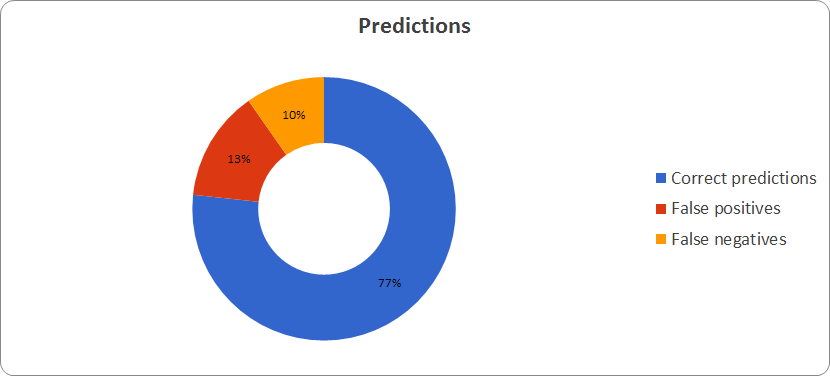
\includegraphics[width = \columnwidth]{Figures/prediction}
	\caption{Predition accuracy of GrandeOmega}
	\label{fig:prediction}
\end{figure}

\begin{figure}[!h]
	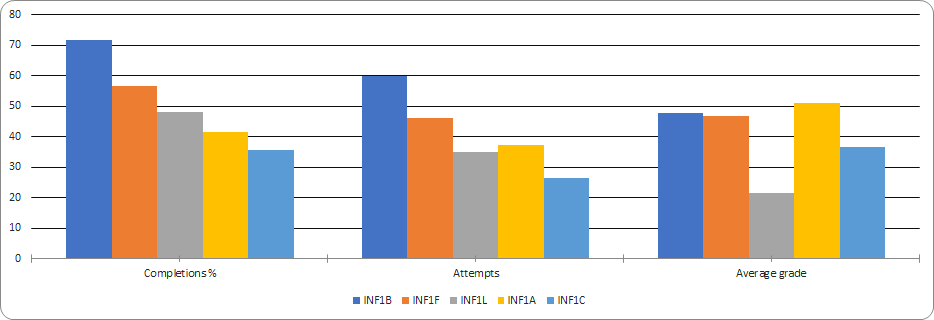
\includegraphics[width = \columnwidth]{Figures/bar_chart}
	\caption{Student performance with and without G.O.}
	\label{fig:bar_chart}
\end{figure}

\section{Conclusions}
\label{sec:conclusions}
%%%%%%%%%%%%%%%%%%%%%%%%%%%%%%%%%%%%%%%%%%%%%%%%%%%%%%%%%%
% conclusions.tex
%%%%%%%%%%%%%%%%%%%%%%%%%%%%%%%%%%%%%%%%%%%%%%%%%%%%%%%%%%

Scripts are an important and pervasive aspect of computer games. Scripts simplify the interaction with computer game engines to the point that a designer or an end-user can easily customize gameplay. Scripting languages must support coroutines because these are a very recurring pattern when creating gameplay modules. Scripts should be fast at runtime because games need to run at interactive framerates. Finally, the scripting runtime should be as modular and as programmable as possible to facilitate its integration in an existing game engine.

In this paper we have shown how to use meta-programming facilities (in particular monads) in the functional language F\# to enhance the existing scripting systems which are based on Lua, the current state of the art, in terms of speed, safety and extensibility. We have also shown how having a typed representation of coroutines promotes building powerful libraries of combinators that abstract many common patterns found in scripts. As evidence of the capabilities of our proposed system we have outlined a series of applications of our scripts into an actual game that is under development.


\end{document}
